\documentclass{../../../template}

\title{CA Lab: Lab 12}

\begin{document}
    \maketitle

    \section*{Task Description}

    We have already written all ofthe components of MIPS Processor:Branch control evaluation unit, general purpose registers, instruction decoder, ALU MEMORY, shifter, signal extension. Now it is time to combine all of our modules and obtain MIPS Processor.

    \section*{Solution}

    The code for the MIPS Processor:

    \lstinputlisting[language=verilog]{../processor.v}

    Here, I used all the modules necessary and cobined them into one Processor (Top Level) module.

    \section*{Simulation and Testing}

    This is the testbench:

    \lstinputlisting[language=verilog]{../testbench.v}

    \begin{figure}[H]
        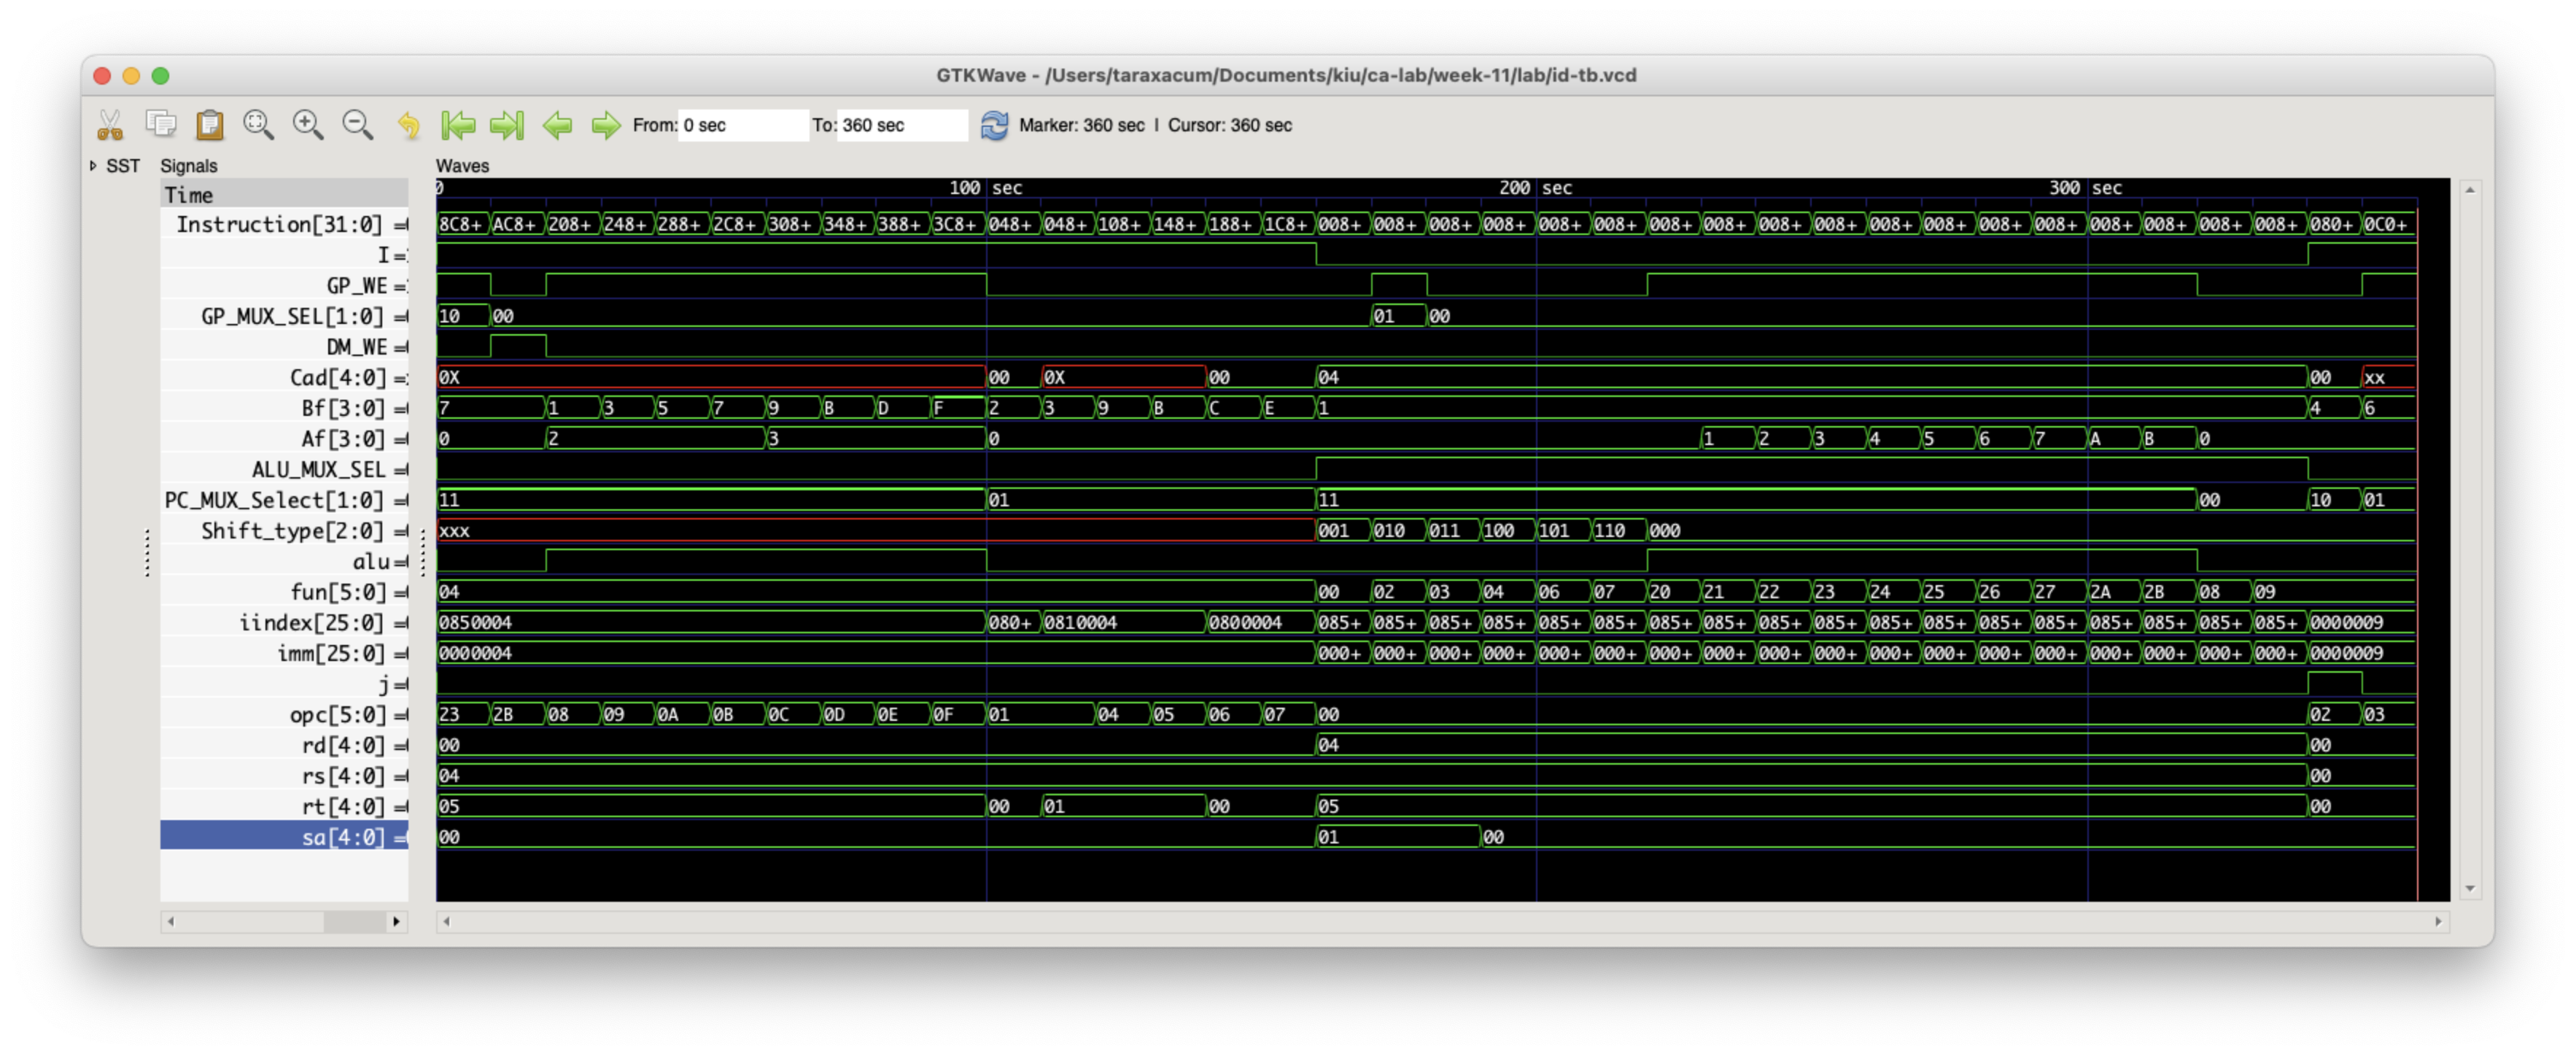
\includegraphics[width=12cm]{diagram.png}
    \end{figure}

    \section*{Reference}

    \begin{itemize}
        \item me
    \end{itemize}
\end{document}